\documentclass[a4paper,twoside]{article}
\usepackage{blindtext}  
\usepackage{geometry}

% Chinese support
\usepackage[UTF8, scheme = plain]{ctex}

% Page margin layout
\geometry{left=2.3cm,right=2cm,top=2.5cm,bottom=2.0cm}


\usepackage{listings}
\usepackage{xcolor}
\usepackage{geometry}
\usepackage{amsmath}
\usepackage{float}
\usepackage{hyperref}

\usepackage{graphics}
\usepackage{graphicx}
\usepackage{subfigure}
\usepackage{epsfig}
\usepackage{float}

\usepackage{algorithm}
\usepackage[noend]{algpseudocode}

\usepackage{booktabs}
\usepackage{threeparttable}
\usepackage{longtable}
\usepackage{listings}
\usepackage{tikz}

% cite package, to clean up citations in the main text. Do not remove.
\usepackage{cite}

\usepackage{color,xcolor}

%% The amssymb package provides various useful mathematical symbols
\usepackage{amssymb}
%% The amsthm package provides extended theorem environments
\usepackage{amsthm}
\usepackage{amsfonts}
\usepackage{enumerate}
\usepackage{enumitem}
\usepackage{listings}

\usepackage{indentfirst}
\setlength{\parindent}{2em} % Make two letter space in the first paragraph
\usepackage{setspace}
\linespread{1.5} % Line spacing setting
\usepackage{siunitx}
\setlength{\parskip}{0.5em} % Paragraph spacing setting

% \usepackage[contents =22920202204622, scale = 10, color = black, angle = 50, opacity = .10]{background}

\renewcommand{\figurename}{图}
\renewcommand{\lstlistingname}{代码} 
\renewcommand{\tablename}{表格}
\renewcommand{\contentsname}{目录}
\floatname{algorithm}{算法}

\graphicspath{ {images/} }

%%%%%%%%%%%%%
\newcommand{\StudentNumber}{22920202204622}  % Fill your student number here
\newcommand{\StudentName}{熊恪峥}  % Replace your name here
\newcommand{\PaperTitle}{作业(六)}  % Change your paper title here
\newcommand{\PaperType}{算法设计与分析} % Replace the type of your report here
\newcommand{\Date}{2022年3月31日}
\newcommand{\College}{信息学院}
\newcommand{\CourseName}{算法设计与分析}
%%%%%%%%%%%%%

%% Page header and footer setting
\usepackage{fancyhdr}
\usepackage{lastpage}
\pagestyle{fancy}
\fancyhf{}
% This requires the document to be twoside
\fancyhead[LO]{\texttt{\StudentName }}
\fancyhead[LE]{\texttt{\StudentNumber}}
\fancyhead[C]{\texttt{\PaperTitle }}
\fancyhead[R]{\texttt{第{\thepage}页,共\pageref*{LastPage}页}}


\title{\PaperTitle}
\author{\StudentName}
\date{\Date}

\lstset{
	basicstyle          =   \sffamily,          % 基本代码风格
	keywordstyle        =   \bfseries,          % 关键字风格
	commentstyle        =   \rmfamily\itshape,  % 注释的风格,斜体
	stringstyle         =   \ttfamily,  % 字符串风格
	flexiblecolumns,                % 别问为什么,加上这个
	numbers             =   left,   % 行号的位置在左边
	showspaces          =   false,  % 是否显示空格,显示了有点乱,所以不现实了
	numberstyle         =   \zihao{-5}\ttfamily,    % 行号的样式,小五号,tt等宽字体
	showstringspaces    =   false,
	captionpos          =   t,      % 这段代码的名字所呈现的位置,t指的是top上面
	frame               =   lrtb,   % 显示边框
}

\lstdefinestyle{PythonStyle}{
	language        =   Python, % 语言选Python
	basicstyle      =   \zihao{-5}\ttfamily,
	numberstyle     =   \zihao{-5}\ttfamily,
	keywordstyle    =   \color{blue},
	keywordstyle    =   [2] \color{teal},
	stringstyle     =   \color{magenta},
	commentstyle    =   \color{red}\ttfamily,
	breaklines      =   true,   % 自动换行,建议不要写太长的行
	columns         =   fixed,  % 如果不加这一句,字间距就不固定,很丑,必须加
	basewidth       =   0.5em,
}

\algnewcommand\algorithmicinput{\textbf{Input:}}
\algnewcommand\algorithmicoutput{\textbf{Output:}}
\algnewcommand\Input{\item[\algorithmicinput]}%
\algnewcommand\Output{\item[\algorithmicoutput]}%

\usetikzlibrary{positioning, shapes.geometric}

\begin{document}
	
%%%%%%%%%%%%%%%%%%%%%%%%%%%%%%%%%%%%%%%%%%%%
\makeatletter % change default title style
\renewcommand*\maketitle{%
	\begin{center} 
		\bfseries  % title 
		{\LARGE \@title \par}  % LARGE typesetting
		\vskip 1em  %  margin 1em
		{\global\let\author\@empty}  % no author information
		{\global\let\date\@empty}  % no date
		\thispagestyle{empty}   %  empty page style
	\end{center}%
	\setcounter{footnote}{0}%
}
\makeatother
%%%%%%%%%%%%%%%%%%%%%%%%%%%%%%%%%%%%%%%%%%%%
	
	
\thispagestyle{empty}

\vspace*{1cm}

\begin{figure}[h]
	\centering
	\includegraphics[width=4.0cm]{logo.png}
\end{figure}

\vspace*{1cm}

\begin{center}
	\Huge{\textbf{\PaperType}}
	
	\Large{\PaperTitle}
\end{center}

\vspace*{1cm}

\begin{table}[h]
	\centering	
	\begin{Large}
		\renewcommand{\arraystretch}{1.5}
		\begin{tabular}{p{3cm} p{5cm}<{\centering}}
			姓\qquad 名 & \StudentName  \\
			\hline
			学\qquad号 & \StudentNumber \\
			\hline
			日\qquad期 & \Date  \\
			\hline
			学\qquad院 & \College  \\
			\hline
			课程名称 & \CourseName  \\
			\hline
		\end{tabular}
	\end{Large}
\end{table}

\newpage

\title{
	\Large{\textcolor{black}{\PaperTitle}}
}
	
	
\maketitle
	
\tableofcontents
 
\newpage
\setcounter{page}{1}

\begin{spacing}{1.2}

\section{题7.3}

首先,要使用尽可能少的教室来调度所有的活动,等价于求最大兼容子集的个数。
所以可以反复调用$GreedyTaskSelect$,然后将选出的兼容子集从原集合中减去。直到所有的活动都被减去。
如算法\ref{algo:assignclass1}

\begin{algorithm}
	\caption{安排教室}
	\label{algo:assignclass1}
	\begin{algorithmic}[1]
		\Input{活动集合A}
		
		\Procedure{AssignClassRoom}{$A$}     
		
		\State $n\gets 0$

		\While{$A$ is not empty}
		\State $S \gets$ \Call{GreedyTaskSelect}{$A$}
		\State $A\gets A-S$
		\State $n\gets n+1$
		\EndWhile

		\State \Return $n$
		
		\EndProcedure
	\end{algorithmic}
\end{algorithm}	

由于$GreedyTaskSelect$有时间复杂度$\mathcal{O}(n)$,设想一个最坏情况,即每一个活动有相同的开始和结束时间,
那么$AssignClassRoom$的时间复杂度就是$\mathcal{O}(n^2)$。因为它调用了$GreedyTaskSelect$共$n$次。

\begin{proof}[证:$AssignClassRoom$有贪心选择性质和最优子结构性质]
	
如果一个教室分配不是最优的,那么存在至少两个教室$C_i$和$C_j$,使得$C_i$和$C_j$的活动集合$A_i$和$A_j$不是最大兼容子集。
设$C_i$较最大兼容子集少,$C_j$包含缺少的元素,那么将$C_j$的元素加入$C_i$,$C_i$就包含最大兼容子集,而教师总数减少$1$

因此任何一个合法的解都能改造成贪心解,使得教室的分配是最优的。该问题有贪心选择性质。

如果在所有活动中移除一个活动$\{S-a_i\}$,假设这个活动被分配到了$C_i$,那么移除之后$C_i$依然包含一个最大兼容子集
可见教室分配的方案依然是每个教室分配一个$\{S-a_i\}$的最大兼容子集的最优解。

因此任何一个解都是由一次贪心选择和一个子问题构成的。该问题有最优子结构性质。

\end{proof}

\section{题7.6}

设一个编码二叉树不是满二叉树,那么不妨设在满二叉树中的某一子树中,应该出现在$i$层的节点$n$出现在了第$i+1$层,
如图~\ref{fig:codingtree}。

\begin{figure}[htbp]
	\centering
	\caption{前缀编码二叉树的某个子树}
	\label{fig:codingtree}
	\subfigure[满编码二叉树的一个子结构]{
		\begin{minipage}[t]{0.4\linewidth}
			\centering
			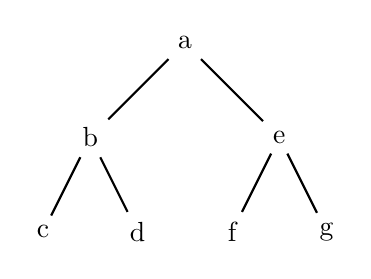
\begin{tikzpicture}
				[thick,scale=0.8, every node/.style={scale=1}]
				\node {a}
				child {node {b}
					child {node {c}}
					child {node {d}}
				}	
				child [missing] {}	
				child {node {e}
					child {node {f}}
					child { node {g}}	
				};
			\end{tikzpicture}
			\label{fig:fulltree}
	\end{minipage}}
	\subfigure[对应的非满二叉树的一个子结构]{
		\begin{minipage}[t]{0.4\linewidth}
			\centering
			\begin{tikzpicture}
				[thick,scale=0.8, every node/.style={scale=1}]
				\node {a}
				child {node {b}
					child {node {c}}
				}	
				child [missing] {}	
				child {node {e}
					child {node {f}}
					child { node {g}
						child {node {d}}
					}	
				};
			\end{tikzpicture}
			\label{fig:notfulltree}
	\end{minipage}}
\end{figure}

如果图~\ref{fig:codingtree}\ref{sub@fig:notfulltree}对应了一种最优编码,那么$n$节点的编码长度$l$是最小的。这时,将节点$n$向上移动到第$i$层,
节点$n$的编码长度将变为$l-1$,这与图~\ref{fig:codingtree}\ref{sub@fig:notfulltree}对应最优编码的假设矛盾。注意到将节点$n$向上移动到第$i$层,
二叉树会变为满二叉树,如图~\ref{fig:codingtree}\ref{sub@fig:fulltree},因此没有一棵非满二叉树对应一个最优前缀编码。

\section{题7.9}

硬币的面值是$1,5,10$,满足
\[2\times 5<1+10
\]

所以贪心算法可以给出最优解。先对硬币面值进行排序,从最大面值起依次进行兑换,如算法~\ref{algo:coin}。

\begin{algorithm}
	\caption{硬币兑换}
	\label{algo:coin}
	\begin{algorithmic}[1]
		\Input{面值$X$,硬币$coins$}
		
		\Procedure{ChangeCoins}{$X,coins$}     
		
		\State \Call{Sort}{$coins$}

		\State $results \gets \varnothing$
		\For{$coin \in coins$}
		\While{$X>0$}
			\State $X \gets X-coin$
			\State $results \gets results \cup coin$
		\EndWhile
		\EndFor

		\State \Return $results$
		
		\EndProcedure
	\end{algorithmic}
\end{algorithm}	

\section{题7.10}

为了使得等待时间最少,可以使用贪心算法。从需要服务时间最少的客户开始服务,可以使得等待时间最少

\begin{itemize}
	\item 贪心选择性质
	\begin{proof}
		假设有服务序列$S$的一个最优解为$A$,$g_k$是$A$中服务时间最短的客户,$g_m$是$S$中服务客户时间最短的客户。
		如果\(g_k=g_m\),则$g_m\in S$,否则,如果\(g_k \neq g_m\),
		则构造$A'$,将$a_k$与$A$中满足$a_i=a_m$的元素交换
		由于$a_m$服务时间最短,所以每一个活动的等待时间不会更长。
		因此$A'$是一个最优解。
	\end{proof}
	\item 最优子结构
	\begin{proof}
		如过$A=\{g_1,g_2,\ldots,g_k,g_{k+1},\ldots\}$是一个最优解且有$g_k>g_{k+1}$,那么交换$g_k$与$g_{k+1}$可以使$g_{k+1}$之后的元素等待时间更少
		这与$A$是最优解矛盾。
	\end{proof}
\end{itemize}

因此可以得到算法~\ref{algo:service}

\begin{algorithm}
	\caption{客户服务}
	\label{algo:service}
	\begin{algorithmic}[1]
		\Input{客户等待时间集合$G$}
		
		\Procedure{Serve}{$G$}     
		
		\State \Call{Sort}{$G$}

		\State $w \gets G$
		\For{$i=1 \to |G|$}
		\State $w[i]=w[i]+w[i-1]$
		\EndFor

		\State $total\gets 0$
		\For{$i=1 \to |G|$}
		\State $total\gets w[i]-w[0]$
		\EndFor
		

		\State \Return $total/|Q|$
		
		\EndProcedure
	\end{algorithmic}
\end{algorithm}	

该算法可以得出最小的平均等待时间。

\section{题7.12}

对于正整数,$y=a^x$和$y=x^a$都有单调不减性。因此将$A,B$倒序排列可以获得最大的回报,如算法~\ref{algo:maxreturn}。

\begin{algorithm}[H]
	\caption{获取最大回报}
	\label{algo:maxreturn}
	\begin{algorithmic}[1]
		\Input{集合$A,B$}
		
		\Procedure{MaxReturn}{$A,B$}     
		
		\State \Call{Sort}{$A,B$}
		
		\State $ret \gets 0$
		\For{$i=0 \to |A|$}
			\State $ret \gets ret + A[i]^{B[i]}$
		\EndFor

		\State \Return $ret$		
		\EndProcedure
	\end{algorithmic}
\end{algorithm}	

该贪心算法可以得到最大回报。

\begin{proof}
	如果一个得到最大回报的排序,对于$B$中的元素存在$b_i<b_j$,不妨设$A$中的元素单调不增,那么在
	\[
		\prod\{a_1^{b_1},a_2{b^2},\ldots,a_i^{b^i},a_j^{b_j},\ldots,a_n^{b_n}\}
	\]
	中交换$b^i$和$b^j$,那么对其他元素幂的乘积大小无影响,而$a_i>a_j,b_j>b_i$,则$a_i^{b^j}\cdot a_j^{b_i}>a_i^{b^i}\cdot a_j^{b_j}$,
	由$y=a^x$的单调不减性,这样整体乘积不会减少,并且将上式改造为了一贪心解,因此贪心算法是正确的。
\end{proof}

\section{题7.14}

$GreedyCaching$算法具有贪心选择性质。
\begin{proof}
	设一个置换出元素在置换出缓存之后再一次访问的时间点的最优序列为
	\[
		E_1,E_2,\ldots,E_n
	\]
	设贪心解为
	\[
		F_1,F_2,\ldots,F_n
	\]
	因为贪心策略选择之后尽可能迟访问的页面,那么$F_1\ge E_1$

	如果$F_1=E_1$,那么不需要改造

	如果$F_1>E_1$,那么将满足$E_1<E_k\le E_k$的元素$E_k$与$E_1$交换,那么由于$E_k>E_1$,
	在整个过程中缓存的置换次数不会增加。进行类似的改造,完全将最优解改造成贪心解,
	而置换次数不会增加,因此贪心解也是一个最优解。它具有贪心选择性质。
\end{proof}

\end{spacing}

\end{document}